\begin{figure}[!h]
	\centering
	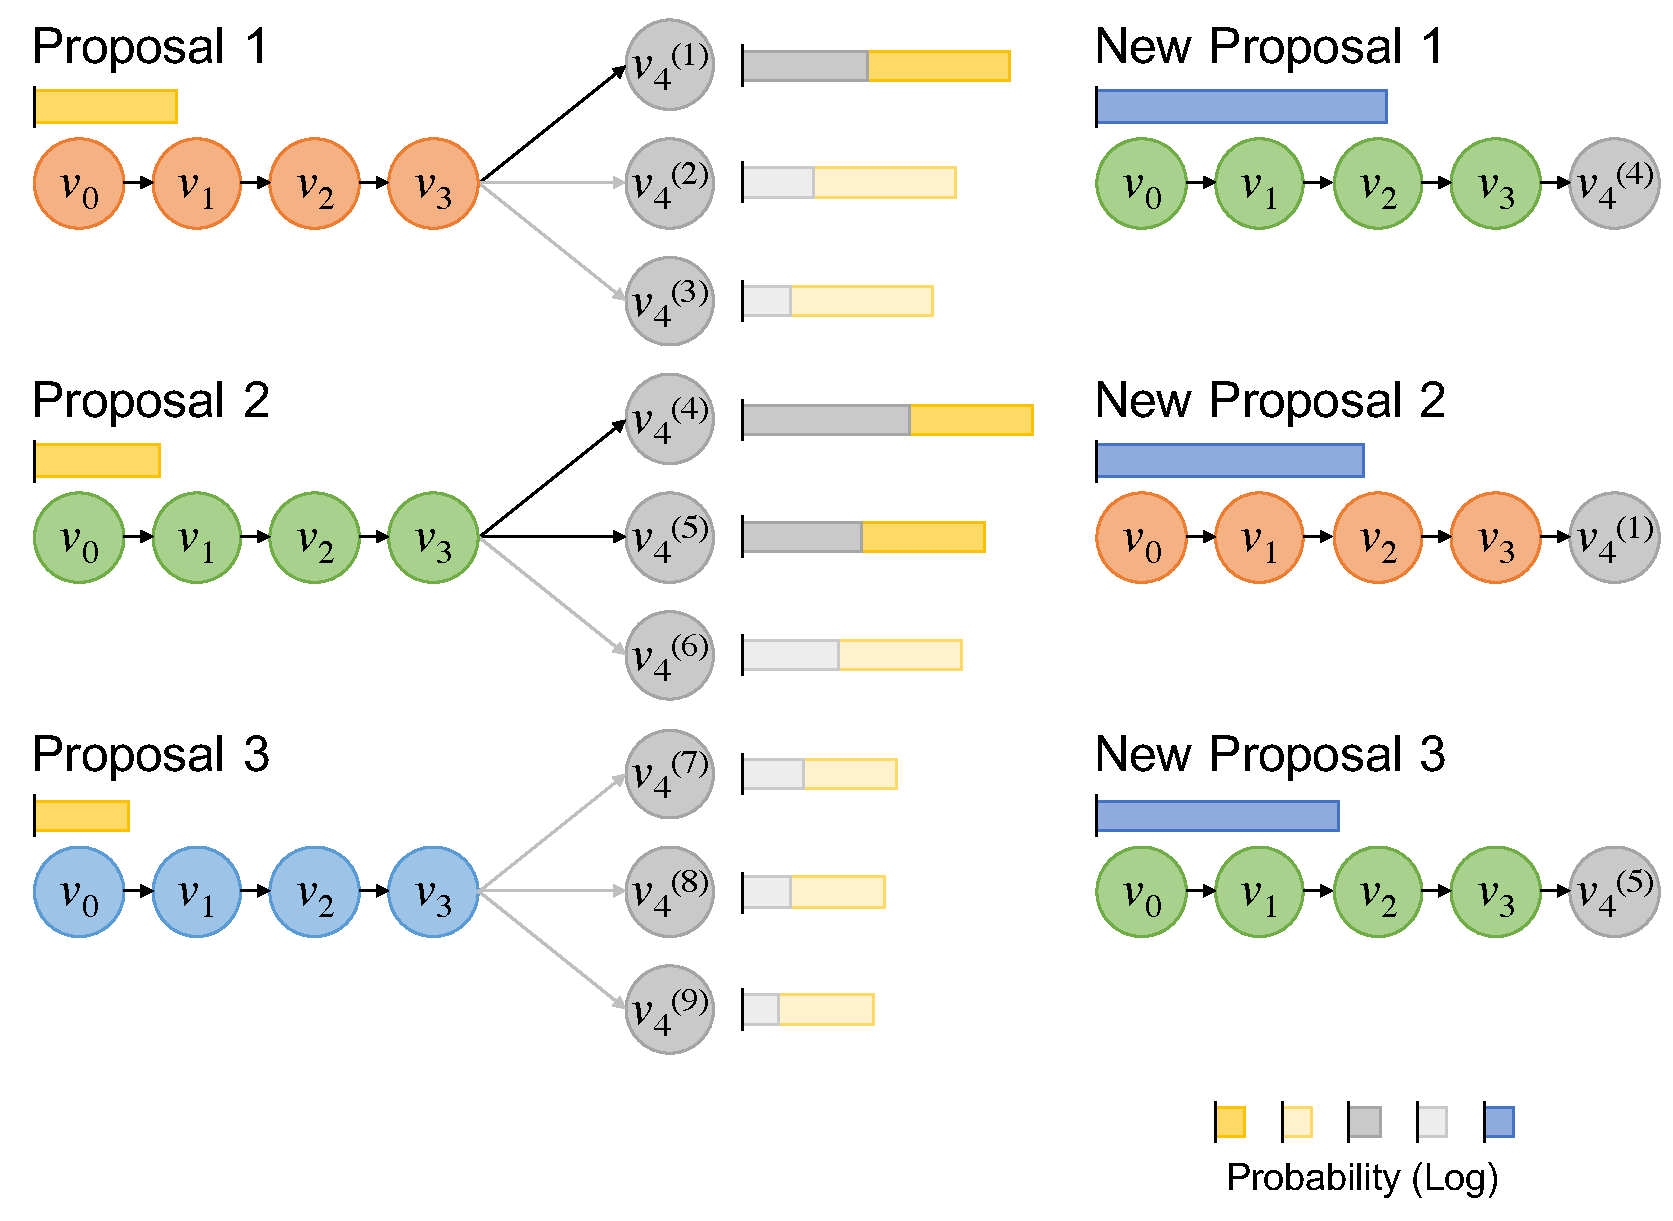
\includegraphics[width=\fig\textwidth]{3-19.pdf}
    \caption[Example of a single step of beam search algorithm]{Example of a single step of beam search algorithm. Suppose currently we have three proposals for the first four vertices, with its corresponding probability (in yellow). For each proposal, we compute the probability distribution (in gray or light gray) for the fifth vertex, and present top three with the highest probability. Totally we have nine possible choices. For each choice, we compute its probability, which is the current one (in gray) plus (here using log probability, thus plus) the previous one. We take top three of these nine choices as our new proposals with new probability (in blue), and continue to the next loop.}
	\label{fig:bmsrch}
\end{figure}

